\documentclass{elegantbook}

\author{ 物理楼\&220 }
\date{\today}
\email{zhaor25@mail2.sysu.edu.cn}
\usepackage{ntheorem}
\usepackage{lstcustom}
\usepackage{listings}
\lstdefinestyle{mystyle}{
    backgroundcolor=\color{backcolour},
    commentstyle=\color{codegreen},
    keywordstyle=\color{magenta},
    numberstyle=\tiny\color{codegray},
    stringstyle=\color{codepurple},
    basicstyle=\footnotesize,
    breakatwhitespace=false,
    breaklines=true,
    captionpos=b,
    keepspaces=true,
    numbers=left,
    numbersep=5pt,
    showspaces=false,
    showstringspaces=false,
    showtabs=false,
    tabsize=2
}


\zhtitle{$mu$子探测实验数据处理补充材料}
%\zhend{模板}
%\entitle{Elegant\LaTeX{} Book}
%\enend{Template}
\version{1.0}
%\myquote{Victory won\rq t come to us unless we go to it.}
\logo{ElegantLaTeX_green.pdf}
\cover{cover.pdf}

%green color
   \definecolor{main1}{RGB}{0,120,2}
   \definecolor{second1}{RGB}{230,90,7}
   \definecolor{third1}{RGB}{0,160,152}
%cyan color
   \definecolor{main2}{RGB}{0,175,152}
   \definecolor{second2}{RGB}{239,126,30}
   \definecolor{third2}{RGB}{120,8,13}
%blue color
   \definecolor{main3}{RGB}{20,50,104}
   \definecolor{second3}{RGB}{180,50,131}
   \definecolor{third3}{RGB}{7,127,128}

\usepackage{makecell}
\usepackage{lipsum}
\usepackage{texnames}

\begin{document}
\maketitle
%\tableofcontents
%\mainmatter
\chapter{数据处理背景简介 }
实验过程中我们给PMT设置合理的高压,设置合理的ADC采集参数,通过ADC模块采集数据并存储到一个lvm格式的文件。这个文件存储了大量(取决于你设置的事件数)的波形信息,我们需要计算每一个信号波形的积分面积,并算出此工作电压下PMT的增益大小。

由于我们要处理的波形数量比较多,需要进行简单的编程来计算和统计;python,MATLAB,C++等都可以满足需求\footnote{可以参考附录的python,ROOT程序}。
\section{读取波形}
我们存储下来的lvm文件每行只有一个数字,代表一个电压值(单位mV);如果你在labview中设置采样长度是1000,那么每1000行就组成一个波形;每一个点的时间间隔是1ns。
\begin{figure}[!htbp]
	\centering
	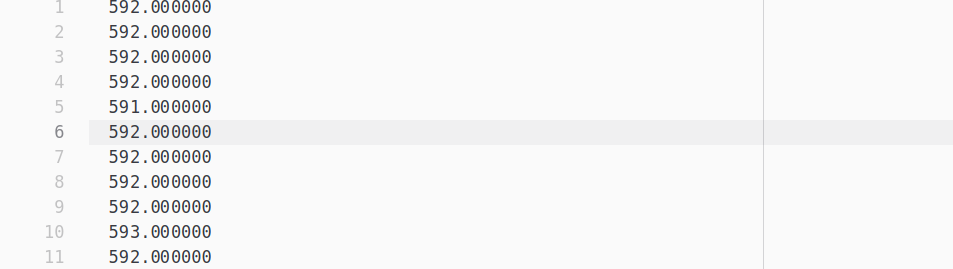
\includegraphics[width=1.016\textwidth]{expdata1.png}
	\caption{lvm 文件\label{fig:g}}
\end{figure}

%\begin{enumerate}[noitemsep]
%   \item 特别修正附录相关内容。
%\end{enumerate}

\section{计算PMT的增益}
数据采集ADC的阻抗是50$\Omega$,我们用波形的面积($\int UT$) 除以电阻可以得到每一个信号的电荷量大小。实验中我们看到的信号来自于$\mu$子在闪烁体中沉积能量产生的发光,我们简单假设每个$\mu$子事件平均产生光子数为5000个,系统总的的探测效率是10\%,那么我们预期看到的PMT信号就是$5000\times 10\%=500$个电子被放大之后的结果。PMT对电子的放大倍数,也就是增益可以用公式\ref{e1}来计算:
\begin{definition}{增益计算}{it}
\begin{equation}
   \label{e1}
	\delta=\frac{Q_{out}}{q}=\frac{\overline{\int UT}}{Rq}.
\end{equation}
\end{definition}
其中$Q_{out}$是放大之后波形的电荷量,q是未经放大的电荷量;我们假设每个事件的平均光电子数为500,也就是$q=500\times e$ 。\footnote{e是电子电荷量}


%\begin{enumerate}[noitemsep]
%   \item 添加一个简化风格(plain)的颜色主题。
%\end{enumerate}

%\chapter{ElegantBook 设置说明}


%\section{编译方式}
%
%本模板基于基础的 book 文类,所以 book 的选项对于本模板也是有效的。默认编码为 UTF-8,推荐使用 \TeX{} Live 编译。作者编写环境为 Win10(64bit) + \TeX{} Live 2018。由于使用的是 \texttt{ctex} 宏包,所以支持 \texttt{pdflatex} 以及 \texttt{xelatex} 编译。
%
%
%\section{选项设置}
%本文特殊选项设置共有 2 类,分为 {\color{main}主题颜色}设置 以及 {\color{main}章标题显示风格}设置。
%
%第 1 类为{\color{main}主题颜色}设置,内置 3 组颜色主题,分别为 \verb|green|(默认)、\verb|cyan|、\verb|blue|,另外还有一个自定义的选项  \verb|nocolor|。调用颜色主题 \verb|green| 的方法为 \\
%\verb|\documentclass[green]{elegantbook}| 或者 \verb|\documentclass[color=green]{elegantbook}|。需要改变颜色的话请选择 \verb|nocolor| 选项或者使用 \verb|color=none|,然后在导言区定义 main、second、third 颜色,具体的方法如下:
%
%\begin{verbatim}
%\definecolor{main}{RGB}{70,70,70}    %定义 main 颜色值
%\definecolor{second}{RGB}{115,45,2}    %定义 second 颜色值
%\definecolor{third}{RGB}{0,80,80}     %定义 third 颜色值
%\end{verbatim}
%
%\begin{table}[htp]
%\caption{ElegantBook 模板中的三套颜色主题\label{tab:color thm}}
%\centering
%\begin{tabular}{ccccc}
%\toprule
%	  & green & cyan & blue & 主要使用的环境\\
%\midrule
%main & \makecell{{\color{main1}\rule{1cm}{1cm}}}& \makecell{{\color{main2}\rule{1cm}{1cm}}}&\makecell{ {\color{main3}\rule{1cm}{1cm}}}& definition \\
%
%second &\makecell{ {\color{second1}\rule{1cm}{1cm}}}& \makecell{{\color{second2}\rule{1cm}{1cm}}}&\makecell{ {\color{second3}\rule{1cm}{1cm}}}&theorem \ lemma \ corollary\\
%
%third &\makecell{ {\color{third1}\rule{1cm}{1cm}}}& \makecell{{\color{third2}\rule{1cm}{1cm}}}&\makecell{ {\color{third3}\rule{1cm}{1cm}}}&proposition\\
%\bottomrule
%\end{tabular}
%\end{table}
%
%第 2 类为{\color{main} 章标题显示风格},包含 \verb|hang|(默认)与 \verb|display| 两种风格,区别在于章标题单行显示(\verb|hang|)与双行显示(\verb|display|),本说明使用了 \verb|hang|。调用方式为 \verb|\documentclass[hang]{elegantbook}| 或者 \verb|\documentclass[titlestyle=hang]{elegantbook}|。
%
%综合起来,同时调用三个选项使用 \verb|\documentclass[color=X,titlestyle=Y]{elegantbook}|。其中 \verb|X| 可以选择 \verb|green|,\verb|cyan|,\verb|blue|,\verb|none|;\verb|Z| 可以选择 \verb|hang| 或者 \verb|display|。
%
%\section{数学环境简介}

%在我们这个模板中,定义了三大类环境
%
%\begin{enumerate}[noitemsep]
%\item 定理类环境,包含标题和内容两部分。根据格式的不同分为3种
%   \begin{itemize}[noitemsep]
%      \item {\color{main}\bfseries definition} 环境,含有一个可选项,编号以章节为单位,颜色为 {\color{main}main};
%      \item {\color{second}\bfseries theorem、lemma、corollary} 环境,颜色为主颜色 {\color{second}second},编号均以章节为单位;
%      \item {\color{third}\bfseries proposition} 环境,含有一个可选项,编号以章节为单位,颜色为 {\color{third}{third}}。
%   \end{itemize}
%\item 示例类环境,有 \textbf{example、exercise} 环境,自动编号,编号以章节为单位。
%\item 证明类环境,有 \textbf{proof、note} 环境,特点是,有引导符或者结尾符,\textbf{note} 环境有引导符号,\textbf{proof} 环境有证明完毕标志。
%\item 结论类环境,有\textbf{conclusion、assumption、property,remark、solution} 环境,三者均以粗体的引导词为开头,和普通段落格式一致。
%\end{enumerate}
%
%\section{可编辑的字段}
%在模板中,可以编辑的字段分别为作者 \verb|\author|、邮箱 \verb|\email|、中文标题 \verb|\zhtitle|、中文标题结尾 \verb|\zhend|、英文标题\verb| \entitle|、英文标题结尾 \verb|\enend|、名言 \verb|\myquote|、版本号 \verb|\version|。并且,可以根据自己的喜好把封面水印效果的 \verb|cover.pdf| 替换掉,以及封面中用到的 \verb|logo.png|。
%
%\section{参考文献}
%
%此模板使用了 Bib\TeX{} 来生成参考文献,默认使用的文献样式 aer 样式。参考文献示例:~\cite{Chen2018} 使用了中国一个大型的 P2P 平台(人人贷)的数据来检验男性投资者和女性投资者在投资表现上是否有显著差异。你可以在谷歌学术,Mendeley,Endnote 中获得文献条目(bib item),然后把它们添加到 \verb|reference.bib| 中。在文中引用的时候,引用它们的键值(bib key)即可。注意需要在编译的过程中添加 Bib\TeX{} 编译。
%
%\chapter{ElegantBook 写作示例}
%
%\section{Lebesgue 积分}
%在前面各章做了必要的准备后,本章开始介绍新的积分。在 Lebesgue 测度理论的基础上建立了 Lebesgue 积分,其被积函数和积分域更一般,可以对有界函数和无界函数统一处理。正是由于 Lebesgue 积分的这些特点,使得 Lebesgue 积分比 Riemann 积分具有在更一般条件下的极限定理和累次积分交换积分顺序的定理,这使得 Lebesgue 积分不仅在理论上更完善,而且在计算上更灵活有效。
%
%Lebesgue 积分有几种不同的定义方式。我们将采用逐步定义非负简单函数,非负可测函数和一般可测函数积分的方式。
%
%由于现代数学的许多分支如概率论、泛函分析、调和分析等常常用到一般空间上的测度与积分理论,在本章最后一节将介绍一般的测度空间上的积分。
%
%\subsection{积分的定义}
%
%我们将通过三个步骤定义可测函数的积分。首先定义非负简单函数的积分。以下设 $E$ 是 $\mathcal{R}^n$ 中的可测集。
%
%
%一个自然的问题是,Lebesgue 积分与我们所熟悉的 Riemann 积分有什么联系和区别?在 4.4 在我们将详细讨论 Riemann 积分与 Lebesgue 积分的关系。这里只看一个简单的例子。设 $D(x)$ 是区间 $[0,1]$ 上的 Dirichlet 函数。即 $D(x)=\chi_{Q_0}(x)$,其中 $Q_0$ 表示 $[0,1]$ 中的有理数的全体。根据非负简单函数积分的定义,$D(x)$ 在 $[0,1]$ 上的 Lebesgue 积分为
%\begin{equation}
%   \label{inter2}
%   \int_0^1 D(x)dx = \int_0^1 \chi_{Q_0} (x) dx = m(Q_0) = 0
%\end{equation}
%即 $D(x)$ 在 $[0,1]$ 上是 Lebesgue 可积的并且积分值为零。但 $D(x)$ 在 $[0,1]$ 上不是 Riemann 可积的。
%
%
%有界变差函数是与单调函数有密切联系的一类函数。有界变差函数可以表示为两个单调递增函数之差。与单调函数一样,有界变差函数几乎处处可导。与单调函数不同,有界变差函数类对线性运算是封闭的,它们构成一线空间。练习题 \ref{exer:43} 是一个性质的证明。
%
%\begin{exercise}\label{exer:43}
%设 $f\in L(\mathcal{R}^1)$,$g$ 是 $\mathcal{R}^1$ 上的有界可测函数。证明函数
%\begin{equation}
%   \label{ex:1}
%   I(t) = \int_{\mathcal{R}^1} f(x+t)g(x)dx \quad t \in \mathcal{R}^1
%\end{equation}
%是 $\mathcal{R}^1$ 上的连续函数。
%\end{exercise}
%
%\begin{theorem}{Fubini 定理}{fubi} 
%(1)若 $f(x,y)$ 是 $\mathcal{R}^p\times\mathcal{R}^q$ 上的非负可测函数,则对几乎处处的 $x\in \mathcal{R}^p$,$f(x,y)$ 作为 $y$ 的函数是 $\mathcal{R}^q$ 上的非负可测函数,$g(x)=\int_{\mathcal{R}^q}f(x,y) dy$ 是 $\mathcal{R}^p$ 上的非负可测函数。并且
%\begin{equation}
%   \label{eq:461}
%   \int_{\mathcal{R}^p\times\mathcal{R}^q} f(x,y) dxdy=\int_{\mathcal{R}^p}\left(\int_{\mathcal{R}^q}f(x,y)dy\right)dx.
%\end{equation}
%(2)若 $f(x,y)$ 是 $\mathcal{R}^p\times\mathcal{R}^q$ 上的可积函数,则对几乎处处的 $x\in\mathcal{R}^p$,$f(x,y)$ 作为 $y$ 的函数是 $\mathcal{R}^q$ 上的可积函数,并且 $g(x)=\int_{\mathcal{R}^q}f(x,y) dy$ 是 $\mathcal{R}^p$ 上的可积函数。而且~\ref{eq:461} 成立。
%\end{theorem}
%
\section{波形和积分}
在example文件中,采样长度是2002ns,也就是每2002点组成一个波形。我们需要算出没有信号时的基线的大小,再用基线值减去对应的信号大小积分出信号的面积。

对于每一个波形,我们都可以计算出一个积分面积,然后算出所有波形\footnote{取决于事件数}积分面积的平均值\footenote{也可以填充直方图进行拟合}作为期望的电荷积分;再利用公式\ref{e1}就可以计算出当前工作电压下的增益大小。
\begin{note}
选择合理的时间范围进行积分,不要让信号超出积分的区间。
\end{note}
\section{电压和增益的关系}
调节不同的PMT工作电压,计算相应的增益大小,可以做出一条增益和电压相关的曲线,并在一定范围内可以用直线对其拟合。
\section{$\mu$子的能量和通量测量}
%通过查询PMT的文档可以得到厂家测出的电压和增益关系,在固定PMT的工作电压时我们可以知道其增益大小。此时可以算出每一个$\mu$子事件产生的电子数,假设PMT收集的电子数与$\mu$子的沉积能量
当我们同时\footnote{信号时间差小于一定范围}在闪烁体两端的PMT看到信号时,我们认为测到了一个$\mu$子的信号,通过统计一定时间的符合计数并结合探测器的有效探测面积就可以估算$\mu$子的通量大小。

\begin{figure}[!htbp]
	\centering
	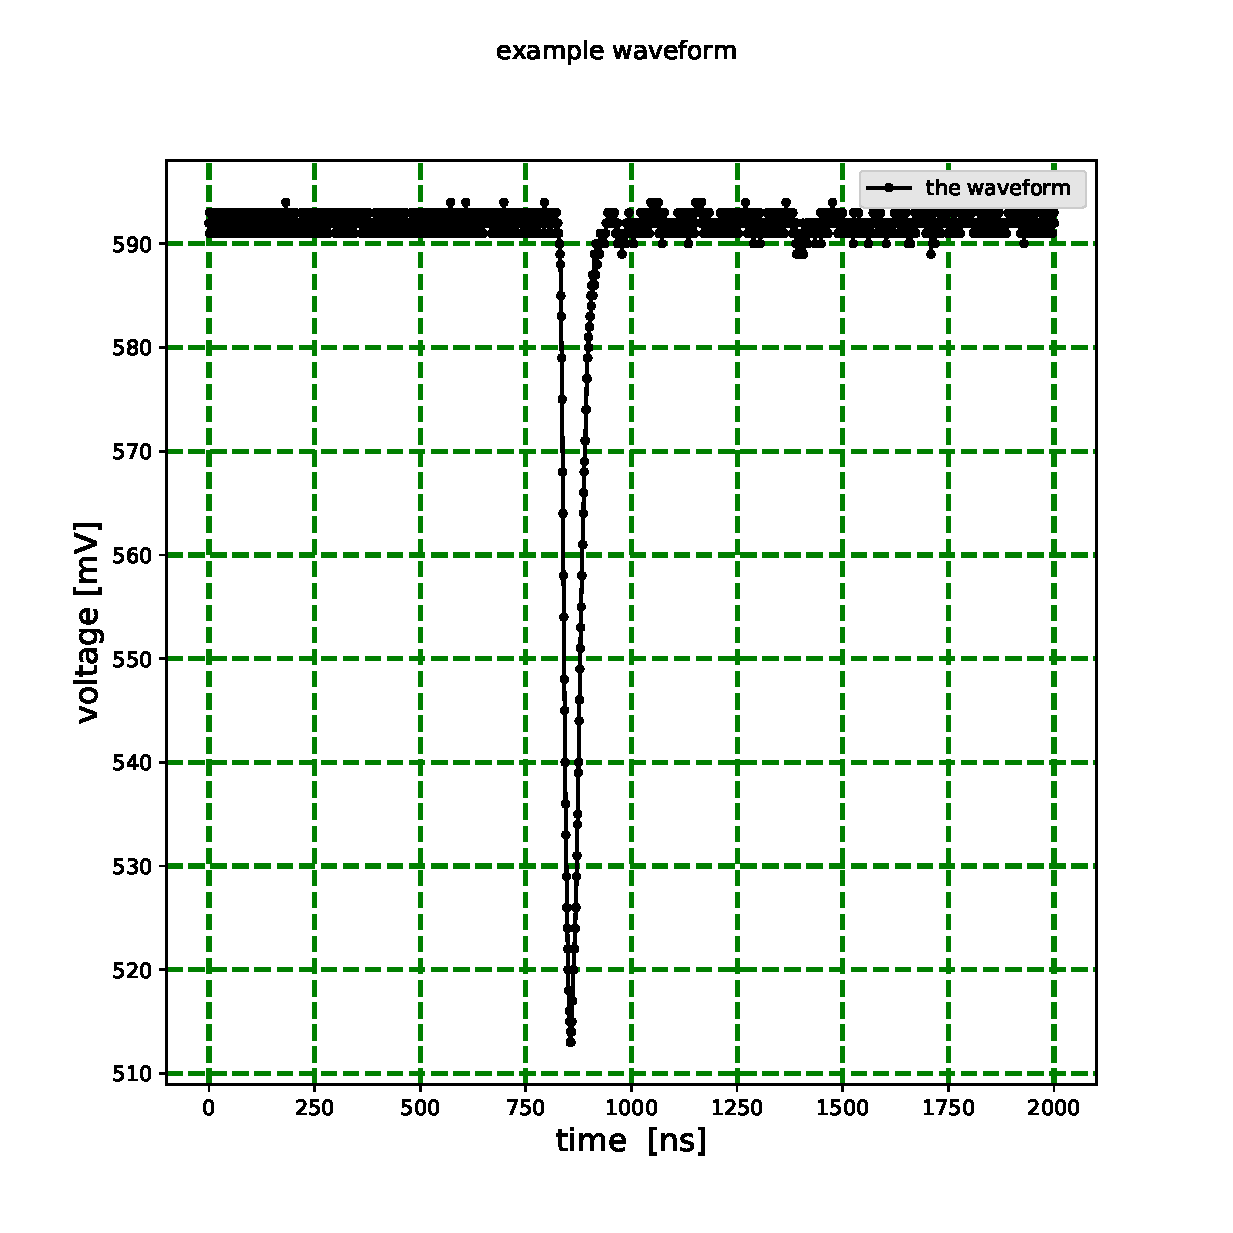
\includegraphics[width=1.016\textwidth]{wave.eps}
	\caption{一个PMT信号波形\label{fig:wave}}
\end{figure}
%
%
%\begin{property}
%柯西列的性质
%\begin{enumerate}[noitemsep]
%\item $\{x_k\}$ 是柯西列,则其子列 $\{x_k^i\}$ 也是柯西列。
%\item $x_k\in \mathcal{R}^n$,$\rho(x,y)$ 是欧几里得空间,则柯西列是收敛的,$(\mathcal{R}^n,\rho)$ 空间是完备的。
%\end{enumerate}
%\end{property}
%

%\begin{conclusion}
%回归分析(regression analysis) 是确定两种或两种以上变量间相互依赖的定量关系的一种统计分析方法。运用十分广泛,回归分析按照涉及的变量的多少,分为一元回归和多元回归分析;按照因变量的多少,可分为简单回归分析和多重回归分析;按照自变量和因变量之间的关系类型,可分为线性回归分析和非线性回归分析。如果在回归分析中,只包括一个自变量和一个因变量,且二者的关系可用一条直线近似表示,这种回归分析称为一元线性回归分析。如果回归分析中包括两个或两个以上的自变量,且自变量之间存在线性相关,则称为多重线性回归分析。
%\end{conclusion}
%
%

\nocite{EINAV2010,Havrylchyk2018} 

%\bibliographystyle{aer}
%\bibliography{reference}

\appendix
\chapter{读取example文件的python程序}

\section{python}
%\begin{listings}
\begin{lstlisting}[caption={A simple listing.}, label={lst:simple}]
#!/usr/bin/env python
# -*-coding:utf-8 -*-
import numpy as np
from scipy import interpolate
import pylab as pl

f = open('/media/tao/_dde_data/arlierwork/simulation/tao/exp220/example.lvm') #换成你自己的文件名
s = f.readline(/media/tao/_dde_data/arlierwork/simulation/tao/exp220)
a1=[]
a2=[]
nevent=1
rec_length=2002   #2002ns 是取数时的采样长度。
count=0
eventnum=0
while (count<rec_length*nevent):  
     arr=s.split(' ')
#     print arr
     a1.append(float(arr[0]))
     a2.append(count)
     s=f.readline()
     count+=1
#print(a1)
#print(a2)
#x=np.linspace(0,10,11)
#x=[  0.   1.   2.   3.   4.   5.   6.   7.   8.   9.  10.]
x=np.array(a1)
y=np.array(a2)
#print(x)


\end{lstlisting}

参考上面的程序,处理多个波形的电荷积分。
\end{document}
